\section{Introduction}

\subsection*{Terminology}
\begin{frame}
\frametitle{Springy Leg Offset Mass}
\begin{columns}
\column{0.5\textwidth}
\begin{figure}
\centering
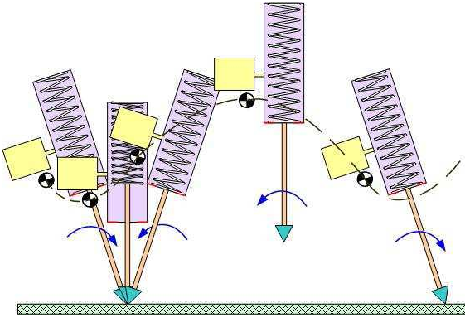
\includegraphics[width=\textwidth]{fig/SLOM_motion.pdf}
\caption{SLOM motion}
\end{figure}

\column{0.5\textwidth}
\begin{block}{Stages}
\begin{itemize}
\item
Lift-off\\[0.1in]
\item
Free fall\\[0.1in]
\item
Touch-down\\[0.1in]
\item
Stance
\end{itemize}
\end{block}
\begin{block}{Terms}
\begin{itemize}
\item
Energy Pumping Mechanism\\[0.1in]
\item
Constraint\\[0.1in]
\item
Energy Release\\[0.1in]
\end{itemize}
\end{block}

\end{columns}
\end{frame}

\subsection*{Aims}
\begin{frame}
\uncover<1->
{
\begin{block}{Design of robot}
\begin{itemize}
  \item Efficient EPM\\[0.1in]
  \item Reaction wheel\\[0.1in]
  \item Onboard electronics
\end{itemize}
\end{block}
}
\uncover<2->
{
\begin{block}{Theory}
\begin{itemize}
  \item Non-linear model\\[0.1in]
  \item Initial conditions\\[0.1in]
  \item In-place hopping\\[0.1in]
  \item Running gait
\end{itemize}
\end{block}
}
\uncover<3->
{
\begin{block}{Experiments}
\begin{itemize}
  \item Attitude estimation\\[0.1in]
  \item Fabrication and interfacing of electronics
\end{itemize}
\end{block}
}
\end{frame}

